%% REPLACE sXXXXXXX with your student number
\def\studentNumber{s1869292}

%% START of YOUR ANSWERS
%% Add answers to the questions below, by replacing the text inside the brackets {} for \youranswer{ "Text to be replaced with your answer." }. 
%
% Do not delete the commands for adding figures and tables. Instead fill in the missing values with your experiment results, and replace the images with your own respective figures.
%
% You can generally delete the placeholder text, such as for example the text "Question Figure 3 - Replace the images ..." 
%
% There are 5 TEXT QUESTIONS. Replace the text inside the brackets of the command \youranswer with your answer to the question.
%
% There are also 3 "questions" to replace some placeholder FIGURES with your own, and 1 "question" asking you to fill in the missing entries in the TABLE provided. 
%
% NOTE! that questions are ordered by the order of appearance of their answers in the text, and not necessarily by the order you should tackle them. You should attempt to fill in the TABLE and FIGURES before discussing the results presented there. 
%
% NOTE! If for some reason you do not manage to produce results for some FIGURES and the TABLE, then you can get partial marks by discussing your expectations of the results in the relevant TEXT QUESTIONS. The TABLE specifically has enough information in it already for you to draw meaningful conclusions.
%
% Please refer to the coursework specification for more details.


%% - - - - - - - - - - - - TEXT QUESTIONS - - - - - - - - - - - - 

%% Question 1: Use Figures 1, 2, and 3 to identify the Vanishing Gradient Problem (which of these model suffers from it, and what are the consequences depicted?). [1/5 of the columns in a 2-column page]
\newcommand{\questionOne} {
  \youranswer{Figure~\ref{fig:grad_flow_08} shows a ``healthy'' gradient flow for VGG08, meanwhile in Figure~\ref{fig:grad_flow_38} we see a prototypical case of the Vanishing Gradient Problem for VGG38. Looking from the output layer (right), leftwards, we see the gradient quickly 'vanishing'; completely undetectable around layer 36 (three from output). The consequnece is shown in the Figure~\ref{fig:curves} training curves, where, VGG08 trains successfully, whereas VGG38 does not even manage to train poorly; it has completely stopped the network from training, ergo no improvement is made from its random initialisation. This totalising obstruction of the Vanishing Gradient Problem historically contributed to why early Deep Neural Networks were not feasible.
  }
}

%% Question 2:
%% Describe Batch Normalization (BN) by using equations. Consider both training and test time and explain how BN addresses the vanishing gradient problem. Note that you are not required to provide the derivation of gradients w.r.t. weights for BN weights. [2/3 of a column in a 2-column page]
\newcommand{\questionTwo} {
%% TODO cut down?
  \youranswer{
    As discussed in Section~\ref{sec:lit_rev}, the Batch Normalisation method (1) normalises\footnote{Sets $\mu=1$ and $\sigma^2=1$, where $\mu$ is the mean and $\sigma^2$ is the varience.} the inputs to a layer for each mini-batch, then (2) uses two new parameters, $\beta$ and $\gamma$, to respectively shift (the mean) and scale (the varience); these are learnt during training, and (3) updates the backprop algorithm to account for the transformed inputs.

    Concretely for a layer $x$ of a network, where $x_{i}^{(k)}$ represents the $k^{th}$ dimension of $x$ for the  $i^{th}$ training example, we have
    \begin{equation}
      \hat{x}_{i}^{(k)}=\frac{x_{i}^{(k)}-\mu_{B}^{(k)}}{\sqrt{\sigma_{B}^{(k)^{2}}+\epsilon}}
    \end{equation}
    where $\mu_{B}^{(k)}$ and $\sigma_{B}^{(k)^{2}}$ are respectively the $k^{th}$ dimension's mean and variance (for batch $B$) and $\epsilon$ is an arbitrarily small constant added to preventing a division by zero.

    The normalisation is then  followed with the rescaling,

    \begin{equation}
      y_{i}^{(k)}=\gamma^{(k)} \hat{x}_{i}^{(k)}+\beta^{(k)}
    \end{equation}

    where $\gamma^{(k)}$, the new mean and $\beta^{(k)}$, the new variance are learned along with the network weights and biases in the ongoing optimisation process. Generally $\beta$ is initialised to 0 and $\gamma$ to 1. This step allows the model to restore its full representational power.

    Overall we have the batchnorm transform,

    \begin{equation}
    B N_{\gamma^{(k)}, \beta^{(k)}}: x_{i}^{(k)} \rightarrow y_{i}^{(k)}
    \end{equation}

    where $m$ is the number of training examples in a mini-batch. Note that $\hat{x}_{i}^{(k)}$ stays internal to the specific layer.

    Finally, the numerous derivations for the back propagation step can be found on page 4 of~\citet{ioffe2015batch}.

    Although Batch Normalisation was not designed specifically to combat the VGP, it is a powerful normalisation and regularisation technique with many use cases. One way it addresses the VGP is by transforming the input to a range that will result a healthy set of gradients for activation functions that 'prefer' inputs within a specified range. For example, the Sigmoid function returns minuscule gradients for numbers of moderately large absolute value (say $\pm3$) and beyond. Its worth noting that batchnorm's lone effectiveness is limited for very deep networks (especially with squishifying activation functions) as repeated multiplication (as taken in gradient backprop) of values less that $|1|$, will tend towards zero
    % * ? Training/ Test Time
  }
}

%% Question 3: Describe Residual Connections (RC) by using equations. Consider both training and test time and explain how RC address the vanishing gradient problem. [1/2 of a column in a 2-column page]
\newcommand{\questionThree} {
  \youranswer{
    ResNets overcome the tendency of networks to degrade in performance\footnote{training performance included; ergo the model is not suffering from overfitting.} past a certain depth (classically 15-30 layers). Residual neural networks do this by utilising skip connections, or shortcuts to jump over some layers.

    % TODO image?
    Formally, given a weight matrix of the form $W^{\ell-k, \ell}$ connecting layer $\ell-k$ to $\ell$ (in our experiments we have stuck to $k=2$), the forwardprop step of our ResNet block is written,

    \begin{equation}
    \begin{aligned}
      y^{\ell} &:=g\left((W^{\ell-1, \ell} \cdot y^{\ell-1}+b^{\ell}) + y^{\ell-k} \right) \\
            &=g\left(\mathcal{F}^{\ell} + y^{\ell-k}\right)
    \end{aligned}
    \end{equation}

    where $y^{\ell}$ is the output of layer $\ell$, $g$ is the activation function,
    $W^{\ell-k, \ell}$ the weight matrix connecting layer $\ell-k$ to $\ell$ and $\mathcal{F}^{\ell}(=W^{\ell-1, \ell} \cdot y^{\ell-1}+b^{\ell})$ is the standard connection before introduction of the shortcut. Note $\mathcal{F}^{\ell}+y^{\ell-k}$ is performed by element-wise addition. If the dimensions of the layers $\ell-k$ and $\ell$ are not equal (as is common in convolution networks due to pooling), we do not add residual connections, however it would be possible to perform a linear projection onto the new dimensions as suggested in the original paper~\cite{he2016deep}.

    A major benefit of ResNets is that they add no parameters or computational complexity. Similarly, the back propagation step is the same for both standard and skipped pathways, essentially unchanged from its classical formulation,

    \begin{equation}
    \begin{aligned}
      \Delta w^{\ell-k, \ell}:&=-\eta \frac{\partial E^{\ell}}{\partial w^{\ell-k, \ell}}\\
                  &=-\eta y^{\ell-k} \cdot \delta^{\ell}
    \end{aligned}
    \end{equation}

    where $\eta$ is the learning rate, $y^{\ell}$ the output from layer $\ell$, and $\delta^{\ell}$ the error at layer $\ell$. As back propagation is of the same form for both the standard and skipped path, the weight matrices are merged and learned in one step (at no additional cost)
  }
}


%% Question 4: Present and discuss the experiment results (all of the results and not just the ones you had to fill in) in Table 1 and Figures 4 and 5 (you may use any of the other Figures if you think they are relevant to your analysis). You will have to determine what data are relevant to the discussion, and what information can be extracted from it. Also, discuss what further experiments you would have ran on any combination of VGG08, VGG38, BN, RC in order to,
%%       \item Improve performance of the model trained (explain why you expect your suggested experiments will help with this).
%%       \item Learn more about the behaviour of BN and RC (explain what you are trying to learn and how).
%% [1 of the columns in a 2-column page]
\newcommand{\questionFour} {
  \youranswer{
    % present results
    % discuss results
  }
}

%% Question 5:
\newcommand{\questionFive} {
\youranswer{Question 5 - Briefly draw your conclusions based on the results from the previous sections (what are the take-away messages?) and conclude your report with a recommendation for future work. 

Good recommendations for future work also draw on the broader literature (the papers already referenced are good starting points). Great recommendations for future work are not just incremental (an example of an incremental suggestion would be: "we could also train with different learning rates") but instead also identify meaningful questions or, in other words, questions with answers that might be somewhat more generally applicable. 

For example, \citep{huang2017densely} end with \begin{quote}``Because of their compact internal representations and reduced feature redundancy, DenseNets may be good feature extractors for various computer vision tasks that build on convolutional features, e.g.,  [4,5].''\end{quote} 

while \cite{bengio1993problem} state in their conclusions that \begin{quote}``There remains theoretical questions to be considered,  such as whether the problem with simple gradient descent  discussed in this paper would be observed with  chaotic attractors that are not  hyperbolic.\\\end{quote}

The length of this question description is indicative of the average length of a conclusion section}
}

%% - - - - - - - - - - - - FIGURES - - - - - - - - - - - - 

%% Question Figure 3:
%% Replace this image with a figure depicting the average gradient across layers, for the VGG38 model.
\newcommand{\questionFigureThree} {
  \youranswer{
    \begin{figure}[t]
        \centering
        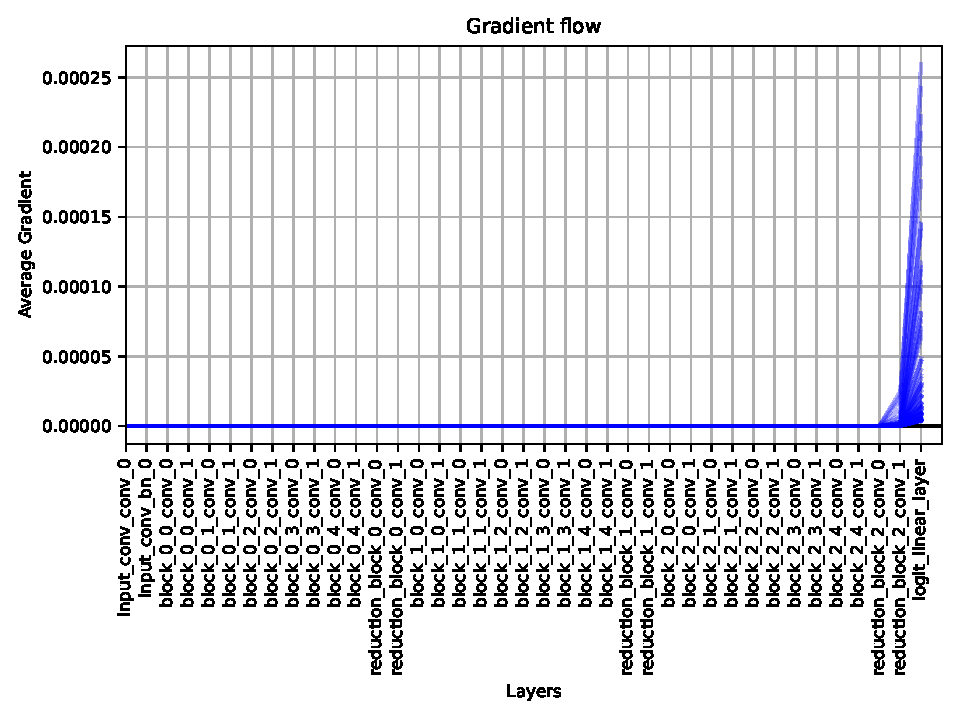
\includegraphics[width=\linewidth]{../VGG_38_experiment/saved_models/gradient_flow_plots/epoch99.pdf}
        \caption{Gradient Flow on VGG38}
        \label{fig:grad_flow_38}
    \end{figure}
  }
}

%% Question Figure 4:
\newcommand{\questionFigureFour} {
\youranswer{Question Figure 4 - Replace this image with a figure depicting the training curves for the model with the best performance across experiments you have available. (Also edit the caption accordingly).
%
\begin{figure}[t]
    \centering
    \includegraphics[width=\linewidth]{example-image-duck}
    \caption{Training curves for ? ? ?}
    \label{fig:grad_flow_bestModel}
\end{figure}
}
}

%% Question Figure 5:
\newcommand{\questionFigureFive} {
\youranswer{Question Figure 5 - Replace this image with a figure depicting the average gradient across layers, for the model with the best performance across experiments you have available. (Also edit the caption accordingly).
%
\begin{figure}[t]
    \centering
    \includegraphics[width=\linewidth]{example-image-duck}
    \caption{Gradient Flow on ? ? ?}
    \label{fig:grad_flow_bestModel}
\end{figure}
}
}

%% - - - - - - - - - - - - TABLES - - - - - - - - - - - - 

%% Question Table 1:
\newcommand{\questionTableOne} {
\youranswer{
Question Table 1 - Fill in Table 1 with the results from your experiments on 
\begin{enumerate}
    \item \textit{VGG38 BN (LR 1e-3)}, and 
    \item \textit{VGG38 BN + RC (LR 1e-2)}.
\end{enumerate}
%
\begin{table*}[t]
    \centering
    \begin{tabular}{lr|ccccc}
    \toprule
        Model                   & LR   & \# Params & Train loss & Train acc & Val loss & Val acc \\
    \midrule
        VGG08                   & 1e-3 & 60 K      &  1.74      & 51.59     & 1.95     & 46.84 \\
        VGG38                   & 1e-3 & 336 K     &  4.61      & 00.01     & 4.61     & 00.01 \\
        VGG38 BN                & 1e-3 & 339 K     &     ?      &     ?     &    ?     &     ? \\
        VGG38 RC                & 1e-3 & 336 K     &  1.33      & 61.52     & 1.84     & 52.32 \\
        VGG38 BN + RC           & 1e-3 & 339 K     &  1.26      & 62.99     & 1.73     & 53.76 \\
        VGG38 BN                & 1e-2 & 339 K     &  1.70      & 52.28     & 1.99     & 46.72 \\
        VGG38 BN + RC           & 1e-2 &     ?     &     ?      &     ?     &    ?     &     ? \\
    \bottomrule
    \end{tabular}
    \caption{Experiment results (number of model parameters, Training and Validation loss and accuracy) for different combinations of VGG08, VGG38, Batch Normalisation (BN), and Residual Connections (RC), LR is learning rate.}
    \label{tab:CIFAR_results}
\end{table*} 
}
}

%% END of YOUR ANSWERS
